% Generated by tools/pipeline/figures.py from a1_dryrun_20260905b/metrics.json. Do not edit by hand.
\begin{figure}[htbp]
\centering
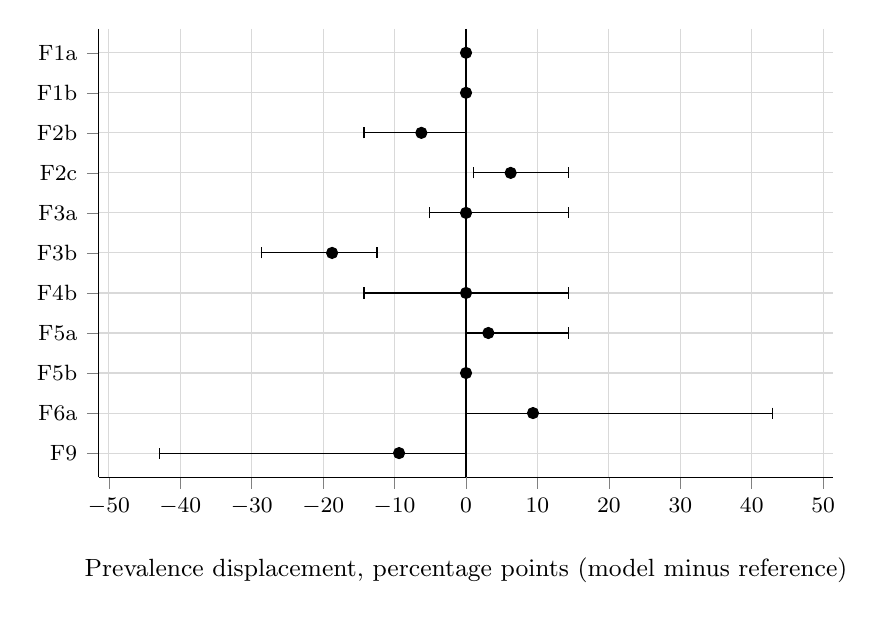
\begin{tikzpicture}
\begin{axis}[
  width=0.9\textwidth, height=0.6\textwidth,
  xlabel={Prevalence displacement, percentage points (model minus reference)}, xlabel style={font=\small},
  symbolic y coords={F1a,F1b,F2b,F2c,F3a,F3b,F4b,F5a,F5b,F6a,F9}, ytick=data, y dir=reverse,
  yticklabel style={font=\footnotesize}, xticklabel style={font=\footnotesize},
  axis lines*=left, tick align=outside, enlarge y limits=0.06, grid=major, grid style={black!15},
  extra x ticks={0}, extra x tick labels={}, extra x tick style={grid=major, grid style={black, thick}},
]
\addplot[only marks, mark=*, mark options={fill=black}, error bars/.cd, x dir=both, x explicit] coordinates {(0.000,F1a) -= (0.000,0) += (0.000,0) (0.000,F1b) -= (0.000,0) += (0.000,0) (-6.250,F2b) -= (8.036,0) += (6.250,0) (6.250,F2c) -= (5.145,0) += (8.036,0) (0.000,F3a) -= (5.126,0) += (14.286,0) (-18.750,F3b) -= (9.821,0) += (6.289,0) (0.000,F4b) -= (14.286,0) += (14.286,0) (3.125,F5a) -= (3.125,0) += (11.161,0) (0.000,F5b) -= (0.000,0) += (0.000,0) (9.375,F6a) -= (9.375,0) += (33.482,0) (-9.375,F9) -= (33.482,0) += (9.375,0)};
\end{axis}
\end{tikzpicture}
\caption{Design-weighted, reference-relative prevalence displacement per frame element in the pooled population: the share of paragraphs on which the model marks the element minus the share on which the reference does, in percentage points of the eligible frame. Bars are the 2.5--97.5 percentile interval over 500 article resamples; no bias-correction estimator is applied. Elements the reference never marks are shown without an interval. Run \texttt{a1\_dryrun\_20260905b}.}
\label{fig:displacement_pooled}
\end{figure}
